\newif\ifembedfigs \embedfigstrue % set \embedfigsfalse for PLOS submission (figures uploaded separately)
\newcommand{\pend}[1]{\textbf{[PENDING: #1]}}
\newcommand{\CI}[2]{[#1,\,#2]}

\begin{document}
\vspace*{0.2in}

\begin{flushleft}
{\Large
\textbf{Ancestra: orthology inference by level-wise reconstruction of ancestral genes inside de novo protein families, and a test of extra data layers}
}
\newline
\\
{}[AUTHORS AND AFFILIATIONS TO BE ADDED BY THE HUMAN ORGANISERS. Text, code and analyses were generated by Claude Opus 5.5 (Anthropic) with Opus/Sonnet 5.5 subagents.]
\end{flushleft}

\section*{Note on how this work was produced}
\textbf{This study was an exercise in testing whether AI agents can run a bioinformatics research project.} An AI agent (Claude Opus 5.5) acted as principal investigator: it planned the work, delegated sub-tasks to other AI agents, ran all analyses and wrote this manuscript. Humans gave the initial task description (S2 Text) and a few later instructions, listed in Materials and methods. \textbf{No human has yet verified the methods or results.} The manuscript should be read as the output of that exercise, not as a peer-reviewed tool paper.

\section*{Abstract}
Most orthology methods either compare every pair of proteomes, build a gene tree for every orthogroup, or place proteins into a precomputed reference database. We tested a different approach. Our method, Ancestra, first splits all proteins into families with a clustering step. It then walks the species tree from the leaves to the root. At each ancestral node it reconstructs the genes of that ancestor, inside every family at once, from mutual best matches, absorbed in-paralogs and small local gene trees. The output is a set of hierarchical orthologous groups (HOGs) in OrthoXML. On the held-out half of OrthoBench (36 reference orthogroups), Ancestra reached F = 76.2, compared with 69.7 for OrthoFinder 3.2, 70.4 for SonicParanoid2, 60.4 for precomputed OMA HOGs and 33.1 for FastOMA, using 3.9 CPU-hours against OrthoFinder's 8.2. The gains over OMA and FastOMA were significant. The gain over OrthoFinder was not: the 95\% interval of the difference, \CI{$-6.5$}{$+18.1$} F points, failed our pre-registered non-inferiority rule. On the Quest for Orthologs 2022 benchmark (78 species), Ancestra matched FastOMA and OMA pairs on TreeFam-A recall but had lower recall than OrthoFinder ($-0.16$), SonicParanoid2 and InParanoid, and the worst species-tree discordance among the main comparators. CPU time grew with the number of proteins to the power 1.16 \CI{1.10}{1.21} up to one million proteins, and to the power 1.35 \CI{1.31}{1.39} from 0.5 to 4.75 million; 1,000 proteomes took 64 CPU-hours but 221 GB of memory. We also tested five extra data layers, and eight more in a second round on development data. Gene order separated orthologs from paralogs well on its own but did not improve the final groups. 3D structure joined more family members but lowered precision. Expression and isoform data did not help, nor did interaction networks, domain architecture or protein language models. Genome sequences showed that 53\% of apparent gene losses in mammals were not real losses. Building HOGs level by level inside families is a viable and scalable approach, but its recall on QfO is still below that of OrthoFinder and the best pairwise methods.

\section*{Author summary}
Genes in different species that descend from one gene in their last common ancestor are called orthologs. Finding them is a basic step in comparing genomes and transferring knowledge between species. As thousands of new genomes appear, orthology methods must be both accurate and fast. We built and tested a method, Ancestra, that reconstructs the genes of each ancestor in the tree of life, one ancestor at a time, inside groups of related proteins. We compared it with leading methods on two standard benchmarks. On OrthoBench it scored higher than OMA-based methods. On the Quest for Orthologs benchmark its recall was similar to that of FastOMA and OMA pairs. It was cheaper than OrthoFinder and ran on 1,000 proteomes on one computer, but it missed more distant orthologs than OrthoFinder and several pairwise methods. Adding gene order, protein structure, expression or isoform data did not improve the final result, even when that data was informative on its own. The work was planned and carried out by AI agents, as a test of how well such agents can run a research project. We report the decisions they took, the methods that failed and the protocol deviations.

\linenumbers

\section*{Introduction}
Orthologs are genes that diverged by speciation; paralogs diverged by duplication~\cite{altenhoff2016qfo}. Hierarchical orthologous groups (HOGs) extend this to many species: a HOG at a taxonomic level contains all genes that descend from one gene of the ancestor at that level~\cite{altenhoff2013gethogs,sarton2025hogreview}. Current methods take one of three routes.
\begin{itemize}
\item \textbf{Pairwise methods} infer orthologs from best hits between every pair of proteomes and then cluster them. Examples are InParanoid~\cite{remm2001inparanoid,persson2022inparanoid}, OrthoInspector~\cite{nevers2019orthoinspector}, SonicParanoid2~\cite{cosentino2024sonicparanoid2}, ProteinOrtho~\cite{klemm2023proteinortho} and OMA pairs~\cite{altenhoff2024oma}. Their search cost grows with the square of the number of proteomes.
\item \textbf{Tree-based methods} build a gene tree for each orthogroup and reconcile it with a species tree. Examples are OrthoFinder~\cite{emms2019orthofinder,emms2026orthofinder3}, PhylomeDB~\cite{fuentes2022phylomedb}, Ensembl Compara~\cite{vilella2009ensemblcompara} and PANTHER~\cite{thomas2022panther}.
\item \textbf{Placement methods} map new proteins onto a precomputed reference. FastOMA, for example, places proteins into OMA HOGs with OMAmer and then refines the HOGs level by level~\cite{majidian2025fastoma,rossier2021omamer}.
\end{itemize}

A fourth idea is older but less used: build HOGs directly, by reconstructing the gene content of each ancestor along the species tree. SYNERGY did this for fungi with sequence and gene order, from one all-against-all comparison of extant genes whose distances it updates as genes are merged~\cite{wapinski2007synergy}. Hieranoid builds an ancestral consensus proteome at each node and searches it against that of the sister clade~\cite{schreiber2013hieranoid,kaduk2017hieranoid2}. SYNERGY's all-against-all search grows quadratically, and Hieranoid's ancestral searches become expensive at deep nodes.

We asked whether this idea can be made scalable, and whether it can compete with current methods. Our method, Ancestra, keeps the ancestor-by-ancestor logic but restricts all work to protein families that are found first, with a fast clustering step. Ancestral genes are never searched again: their similarity scores are aggregated from the scores of their member proteins, as in SYNERGY~\cite{wapinski2007synergy}.

We also asked whether data beyond the protein sequence helps. Gene order (synteny), 3D structure, expression, alternative isoforms and genome sequences have each been proposed or used as orthology evidence~\cite{lechner2014poff,ludwig2024orthorefine,moi2025foldtree,bastian2025bgee,kirilenko2023toga}. We tested each layer first on its own and then inside the full method, with shuffled controls.

Finally, this project was a test of AI agents. One agent acted as principal investigator and delegated work to other agents, under a pre-registered protocol and a 48-hour budget. We describe this setup in Materials and methods.

\section*{Results}

\subsection*{Overview of the method}
Ancestra has three stages (Fig~\ref{fig:method}).

\textbf{S0: family partition.} DIAMOND clusters all proteins at 30\% identity~\cite{buchfink2021diamond,buchfink2026deepclust}. Then every protein is searched against the cluster representatives, and families are the connected components of hits with at least 30\% coverage. Components larger than 7,500 proteins are split with the Leiden algorithm~\cite{traag2019leiden}. This second step was the key design decision for S0. One clustering pass placed at most 59\% of development reference orthogroups into a single family, because representatives of one family are often too distant to hit each other. Searching all proteins against the representatives raised this to 79\%.

\textbf{S2: scoring inside families.} DIAMOND compares proteins within each family. MMseqs2~\cite{steinegger2017mmseqs2} then re-aligns the within-family pairs that DIAMOND missed (6--10\% of pairs on simulated data). The score of a pair is its bit score divided by the larger self-score.

\textbf{S3: level-wise merge.} Ancestra walks the NCBI taxonomy tree~\cite{schoch2020ncbitaxonomy}, restricted to the input species, from the leaves to the root. Each internal node can have more than two children. At each node, and in every family at once, it merges the ancestral genes of the child clades into ancestral genes of the node:
\begin{enumerate}
\item Ancestral genes from different children that are mutual best matches (within a tolerance of 0.95) become orthologs. This is the reciprocal-best-hit rule~\cite{remm2001inparanoid}.
\item A gene from the same child that is closer to an ortholog than that ortholog's best cross-child partner joins as an in-paralog. This is the InParanoid rule~\cite{remm2001inparanoid}, as used in Hieranoid~\cite{schreiber2013hieranoid}.
\item Where several near-equal candidates compete, at nodes that are divergent and have an outgroup, a small gene tree decides. The default (\texttt{accurate} preset) aligns one representative per ancestral gene with FAMSA~\cite{deorowicz2016famsa} and builds a tree with FastTree~\cite{price2010fasttree2}, as OrthoFinder~3 also does~\cite{emms2026orthofinder3}; FastOMA uses MAFFT and FastTree~\cite{majidian2025fastoma}. The \texttt{fast} preset uses neighbour joining~\cite{saitou1987nj}. Nodes of the tree are labelled duplications or speciations by species overlap~\cite{huertacepas2007overlap}.
\item At deep nodes (median seed score $-\ln S \geq 1.5$), ancestral genes with disjoint species sets are also merged, to reduce false splits at the last common ancestor.
\end{enumerate}
Scores between ancestral genes are the average of the scores between their member proteins, which the method maintains exactly as groups are merged. Ancestral genes that find no partner pass up unchanged. The output is OrthoXML~\cite{schmitt2011orthoxml} with one HOG per ancestral gene and level, plus ortholog pairs and orthogroups. Every output passes a validity check (schema, each gene once, consistent levels, parsing with pyHam~\cite{train2019pyham}).

\textbf{Optional gene-order layer.} If gene positions are given, each ancestral gene inherits the neighbours of its members. Synteny support then re-ranks candidate partners in step 1, but only within the root HOG found without gene order. We added this constraint after unconstrained use fused orthogroups (S1 Text, section 7).

What is new is the combination: HOGs are reconstructed level by level across all families at once, without a reference database, without an all-against-all search and without searching ancestral genes again. The merge rules themselves (mutual best hits, in-paralog absorption, local trees, species overlap) are borrowed. The deep-node rule is a heuristic that we tuned on development data.

\ifembedfigs
\begin{figure}[!h]
\centering
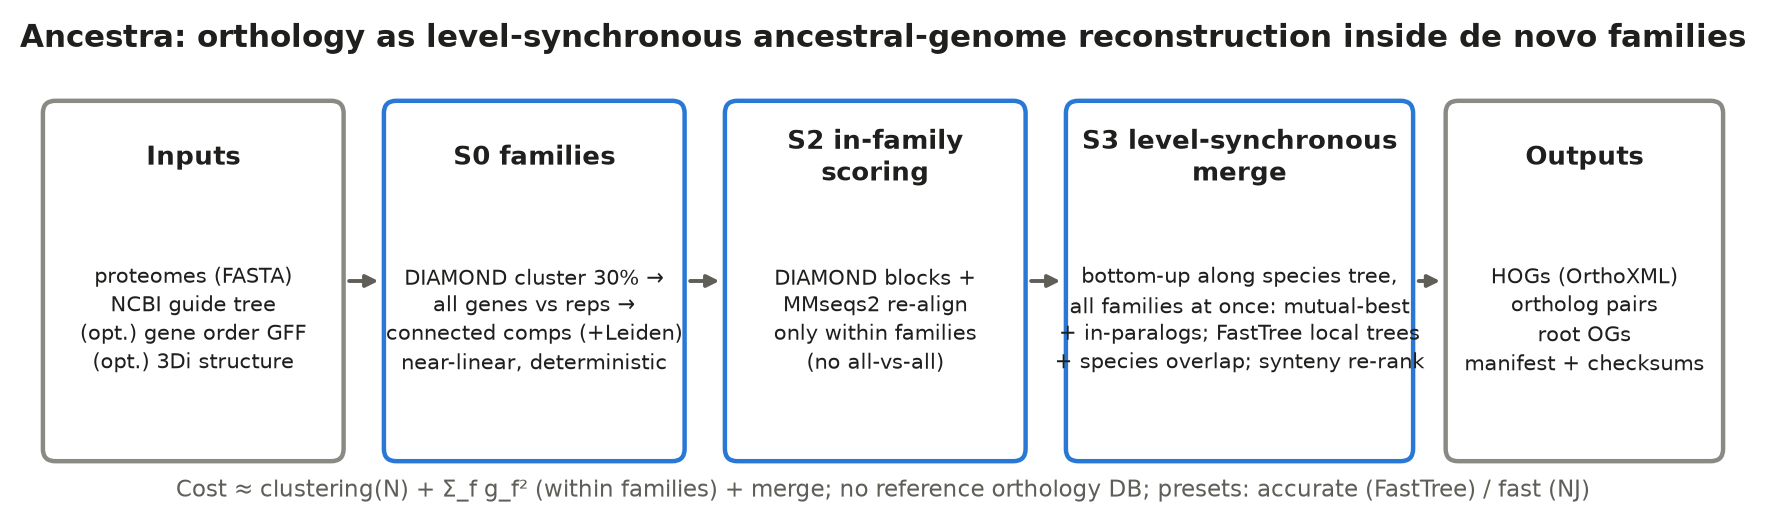
\includegraphics[width=\linewidth]{../docs/figures/fig1_method.png}
\caption{{\bf Overview of Ancestra.} S0 partitions proteins into families; S2 scores pairs within families; S3 walks the guide tree from leaves to root and reconstructs ancestral genes at each node. Optional layers: gene order (re-ranking inside root HOGs), 3Di structure (family rescue, off by default) and genome DNA (validation of gene losses).}
\label{fig:method}
\end{figure}
\fi

\subsection*{Accuracy on OrthoBench}
We split the 70 OrthoBench reference orthogroups (RefOGs)~\cite{trachana2011orthobench,emms2020orthobench} into a development half (34) and a test half (36). The split followed homology components, so that paralogous RefOGs never straddle the two halves. All tuning used the development half. The frozen method was scored once on the test half (Table~\ref{tab:ob}).

\begin{table}[!ht]
\begin{adjustwidth}{-2.25in}{0in}
\centering
\caption{{\bf OrthoBench test results (36 RefOGs).}}
\begin{tabular}{lrrrrr}
\hline
Method & F & Precision & Recall & CPU-h & $\Delta$F (Ancestra $-$ method) [95\% CI]\\
\hline
Ancestra, \texttt{accurate} & 76.2 & 69.5 & 84.2 & 3.9 & --- \\
Ancestra, \texttt{fast} & 74.8 & 68.7 & 82.1 & 2.9 & $+1.4$ \CI{$-3.6$}{$+7.1$}\\
OrthoFinder 3.2 & 69.7 & 62.1 & 79.5 & 8.2 & $+6.5$ \CI{$-6.5$}{$+18.1$}\\
SonicParanoid2 & 70.4 & 70.8 & 70.1 & 7.9 & $+5.7$ \CI{$-4.3$}{$+14.9$}\\
OMA browser HOGs$^a$ & 60.4 & 88.9 & 45.8 & n/a & $+15.7$ \CI{$+1.8$}{$+29.2$}\\
ProteinOrtho & 47.5 & 97.7 & 31.4 & 1.6 & $+28.7$ \CI{$+13.1$}{$+41.9$}\\
FastOMA 0.5.1, patched$^a$ & 33.1 & 23.9 & 53.8 & 19.9 & $+43.1$ \CI{$+14.0$}{$+55.3$}\\
\hline
\end{tabular}
\begin{flushleft}F, precision and recall: official OrthoBench scores, in percent. $\Delta$F: paired bootstrap over RefOGs (2,000 resamples). CPU time is from single runs on a shared node and is indicative only; Ancestra used 10 threads and the competitors 8. The FastOMA CPU time excludes about 0.75 CPU-hours of OMAmer placement reused from the unpatched run. Ancestra rows use the gene-order layer; without it, test F was 76.1 (\texttt{accurate}) and 74.8 (\texttt{fast}). $^a$OMA contains all 12 OrthoBench species, so the OMA-based results are not independent of the benchmark.
\end{flushleft}
\label{tab:ob}
\end{adjustwidth}
\end{table}

Ancestra had the highest F. It was significantly better than the precomputed OMA HOGs, FastOMA and ProteinOrtho. Against OrthoFinder and SonicParanoid2 the point estimates favoured Ancestra by 6.5 and 5.7 points, but the confidence intervals included losses larger than our pre-registered non-inferiority margin of 3 points. We therefore cannot claim that Ancestra is at least as good as OrthoFinder on this benchmark: 36 RefOGs are too few. On all 70 RefOGs, which include the development half and are therefore optimistic, the difference was $+7.8$ \CI{$+0.5$}{$+15.1$}.

FastOMA scored poorly. While investigating this, we found a bug in FastOMA 0.5.1 that dropped 5,497 genes when HOGs were split. We patched it and re-ran FastOMA. Gene coverage rose from 79.0\% to 80.6\%, but test F did not change (33.5 to 33.1). The low score has two sources. Precision was low (23.9), because reference orthogroups were fused into larger HOGs, and 19\% of proteins were missing from FastOMA's groups. In the unpatched run, 9.1\% of proteins were never placed in a FastOMA family and 9.7\% were left as root-level singletons; OMAmer itself left only 4.1\% unplaced. This is consistent with the fusion rate reported for FastOMA on OrthoBench by Emms et al.~\cite{emms2026orthofinder3}. The precomputed OMA browser HOGs are a fairer OMA reference: they were precise (88.9) but had low recall (45.8).

\subsection*{Accuracy on Quest for Orthologs 2022}
We ran the full Quest for Orthologs (QfO) 2022 benchmark suite locally~\cite{altenhoff2024qfo}. To validate our local setup, we re-scored 10 of the 20 published submissions on SwissTree, TreeFam-A and VGNC and reproduced all 60 published TPR/PPV values exactly. The reference set has 78 species and 988,778 proteins. Table~\ref{tab:qfo} shows the main endpoints. S1 Table has all 20 published QfO 2022 methods, both Ancestra presets and all benchmarks.

\begin{table}[!ht]
\begin{adjustwidth}{-2.25in}{0in}
\centering
\caption{{\bf Quest for Orthologs 2022, main endpoints.}}
\begin{tabular}{lcccc}
\hline
Method & SwissTree TPR/PPV & TreeFam-A TPR/PPV & EC (n, thousands) & G-STD2 Euk. RF (n)\\
\hline
Ancestra, \texttt{accurate} & 0.721/0.926 & 0.583/0.921 & 0.899 (181) & 0.257 (3,379)\\
Ancestra, \texttt{fast} & 0.731/0.923 & 0.608/0.916 & 0.896 (197) & 0.266 (4,753)\\
OrthoFinder & 0.825/0.917 & 0.737/0.918 & 0.931 (204) & 0.249 (6,629)\\
SonicParanoid2 (sens-g) & 0.717/0.938 & 0.667/0.936 & 0.906 (222) & 0.232 (4,878)\\
Hieranoid 2 & 0.726/0.950 & 0.621/0.930 & 0.948 (169) & 0.222 (3,643)\\
InParanoid 5 & 0.701/0.944 & 0.627/0.933 & 0.927 (198) & 0.227 (3,655)\\
FastOMA (v0.1.4) & 0.699/0.953 & 0.546/0.919 & 0.928 (157) & 0.239 (3,092)\\
OMA HOGs & 0.696/0.924 & 0.580/0.923 & 0.829 (308) & 0.237 (2,981)\\
OMA pairs & 0.677/0.929 & 0.565/0.920 & 0.952 (156) & 0.226 (2,369)\\
\hline
\end{tabular}
\begin{flushleft}TPR, PPV: recall and precision of reference ortholog pairs. EC: average Schlicker similarity of EC numbers between predicted orthologs. G-STD2: Robinson--Foulds distance (lower is better) between gene trees from predicted orthologs and the species tree, with the number of trees in brackets. Competitor values are published submissions. Ancestra rows use the gene-order layer.
\end{flushleft}
\label{tab:qfo}
\end{adjustwidth}
\end{table}

We pre-registered TreeFam-A recall on held-out families as a primary endpoint. A paired bootstrap over the 749 held-out TreeFam-A families gave these differences in recall for \texttt{accurate}:
\begin{itemize}
\item vs FastOMA: $+0.043$ \CI{$-0.005$}{$+0.093$}, non-inferior;
\item vs OMA pairs: $+0.018$ \CI{$-0.028$}{$+0.069$}, non-inferior;
\item vs OMA HOGs: $+0.002$ \CI{$-0.058$}{$+0.067$}, inconclusive;
\item vs OrthoFinder: $-0.160$ \CI{$-0.210$}{$-0.106$}, inferior;
\item vs Hieranoid 2: $-0.036$ \CI{$-0.069$}{$+0.004$}, not shown non-inferior;
\item vs InParanoid 5: $-0.042$ \CI{$-0.081$}{$-0.000$}, lower, not non-inferior;
\item vs SonicParanoid2 (sens-g): $-0.087$ \CI{$-0.132$}{$-0.038$}, inferior.
\end{itemize}
OrthoFinder, FastOMA, Hieranoid 2, InParanoid 5 and SonicParanoid2 were the pre-registered primary comparators. We added OMA pairs and OMA HOGs after a human instruction to include an OMA resource in every comparison. On TreeFam-A precision, non-inferiority was shown only against OMA pairs and OMA HOGs. On SwissTree, recall was also lower than OrthoFinder's ($-0.103$ \CI{$-0.177$}{$-0.029$}). Ancestra had the highest G-STD2 Eukaryota discordance of the methods in Table~\ref{tab:qfo} and lower EC consistency than OrthoFinder.

On QfO, Ancestra therefore sits with the OMA methods: precise, with moderate recall. Why does it lead on OrthoBench but trail on QfO? OrthoBench scores whole orthogroups in 12 mostly bilaterian species. QfO rewards pairwise recall across all eukaryotes and prokaryotes. When we diagnosed recall on development families, 78\% of missed ortholog pairs were split at the pair's last common ancestor. These are mostly deep nodes (Bilateria 34\%, Eukaryota 21\% and Opisthokonta 13\% of these misses), where an outgroup is often missing or distant, so an old duplication is hard to tell from a speciation. Rules that recovered recall at these nodes also fused OrthoBench orthogroups (S1 Text, section 4.7). We did not resolve this trade-off.

\subsection*{Effect of extra data layers}
We tested each layer in two steps: first on its own sub-task benchmark with a shuffled control, then inside the frozen method on held-out data (Table~\ref{tab:layers}).

\begin{table}[!ht]
\begin{adjustwidth}{-2.25in}{0in}
\centering
\caption{{\bf Effect of extra data layers.}}
\begin{tabular}{p{2.3cm}p{4.6cm}p{3.8cm}p{2.0cm}}
\hline
Layer & On its own (development data) & In the full method (held-out) & Decision\\
\hline
Gene order & Ortholog vs paralog AUC 0.92 human--mouse, 0.49 human--fly; shuffled 0.50 & OrthoBench $\Delta$F $-0.1$ \CI{$-0.4$}{$0.0$} when removed; QfO TreeFam-A (\texttt{fast}) $-0.012$ \CI{$-0.028$}{$+0.001$} & option, no measurable gain\\
3D structure (3Di) & Family completeness 0.794 $\to$ 0.853 (shuffled 0.794) & OrthoBench F $-5.0$ \CI{$-13.1$}{$0.0$}; precision 69.5 $\to$ 60.1 & option, off\\
Expression (Bgee) & AUC 0.667; hard cases $-0.019$ \CI{$-0.20$}{$+0.15$} & not run & rejected\\
Isoforms & AUC 0.760 vs 0.759; hard cases $+0.013$ \CI{$-0.018$}{$+0.044$} & not run & rejected\\
Genome DNA & 92\% recovery of planted controls; 0/512 false hits & validation only & add-on\\
\hline
\end{tabular}
\label{tab:layers}
\end{adjustwidth}
\end{table}

\textbf{Gene order} was the strongest layer on its own. Between closely related vertebrates it separated orthologs from paralogs with AUC 0.92, and it decided 70 of 157 hard cases with precision 0.84. Inside the frozen method, however, it changed neither OrthoBench nor QfO measurably. On development data it had added 1.0 (\texttt{accurate}) to 4.4 (\texttt{fast}) F points; this gain did not replicate. Our reading is that local gene trees and species-overlap rules already resolve the cases where gene order is informative. Gene order carries no signal at deep nodes, where Ancestra loses recall (human--fly AUC 0.49).

\textbf{3D structure.} We used Foldseek 3Di sequences~\cite{vankempen2024foldseek} for 94.5\% of QfO proteins, taken from AlphaFold DB~\cite{varadi2024alphafolddb}. Structure search rejoined family members that sequence search missed, raising family completeness above the ceiling of 0.82 for any partition built from sequence hits. But the rejoined proteins were mostly not true members of the reference orthogroups: OrthoBench precision fell from 69.5 to 60.1. Inside the merge, 3Di scores ranked orthologs above paralogs \emph{worse} than sequence did (AUC 0.694 vs 0.751 at deep nodes), because paralogs share the fold. Structure detects homology but does not separate orthologs from paralogs.

\textbf{Expression and isoforms} failed their pre-registered rules. Expression conservation was weak evidence (AUC 0.667) and was wrong more often than sequence on the paralog cases it was meant to resolve. Choosing the best isoform pair instead of the canonical one changed almost nothing and cost 2--5 times more search.

\textbf{Genome DNA.} We searched the genomes of 2,523 apparent gene losses in mammals with miniprot~\cite{li2023miniprot}, at the locus predicted by gene order. Of these losses:
\begin{itemize}
\item 53\% were not losses. Of all apparent losses, 32\% were errors of our own method (the gene was annotated but placed in another HOG), 19\% were intact but unannotated genes or gene-model errors, and 2\% were relocated copies;
\item 25\% were confirmed losses (pseudogenes or deletions), including the known \textit{UOX} pseudogene in human (\textit{GULO}, which is missing in both human and chimpanzee, was confirmed as a pseudogene by a separate clade-level search);
\item 21\% were unresolved.
\end{itemize} Genome sequence is therefore useful to audit the gene losses implied by HOGs, rather than as an input to inference.

\textbf{Second round of layers.} After the freeze, we tested further layers under one shared protocol, on development data only (Table~\ref{tab:layers2}). Each layer's arms and keep rule were committed before its integration results. Some layers later added post hoc arms, which were logged as deviations. Each layer was compared with shuffled controls, with the exceptions listed in S1 Text, section 10. No arm passed, so none was run on test data.

\begin{table}[!ht]
\begin{adjustwidth}{-2.25in}{0in}
\centering
\caption{{\bf Second round of data layers (development data only).} AUC is for ortholog vs paralog pairs (shuffled controls $\approx$0.50); ``hard'' marks pairs where a paralog scores within 0.9 of the ortholog.}
\begin{tabular}{p{3.4cm}p{5.4cm}p{4.6cm}}
\hline
Layer & On its own & Inside the merge\\
\hline
Interaction networks (STRING, own-species evidence only~\cite{szklarczyk2023string}; hu.MAP 3.0~\cite{fischer2025humap3}) & AUC 0.63 all pairs, 0.50 hard (OrthoBench, 3.4\% of candidates covered); 0.62 and 0.57 (TreeFam-A) & not run; as recall rescue, added pairs were orthologs only 48--54\% of the time\\
Protein abundance (PaxDb~\cite{huang2023paxdb}) & AUC 0.68 all pairs; right in 39 of 116 hard decisions & not run\\
Domain architecture (Pfam~\cite{paysanlafosse2025pfam}) & AUC 0.64 hard (sequence 0.74); 0.98 between orthogroups but 0.54 within one & TreeFam-A F1 $+0.018$ \CI{$+0.003$}{$+0.034$}, but PPV $-0.025$ and OrthoBench OG-F $-2.9$\\
Protein language models (ESM-2~\cite{lin2023esm2}, ProtT5~\cite{elnaggar2022prottrans}) & above shuffled on all pairs, not clearly on hard ones; below sequence everywhere; mostly below chance where sequence fails & not run\\
Contrastive model trained on our own synteny-supported pairs & $+0.040$ \CI{$+0.010$}{$+0.056$} over raw embeddings on all pairs; $-0.007$ \CI{$-0.065$}{$+0.056$} on hard cases & not run\\
Intron positions & AUC 0.58 hard (sequence 0.65); as tie-breaker $-0.071$ \CI{$-0.149$}{$+0.007$} & not run\\
Gene order: repair of split HOGs & 29--40\% fewer fission candidates (shuffled: no change) & macro pair F1 $+0.006$ \CI{$-0.002$}{$+0.016$}; TreeFam-A TPR $+0.004$ \CI{$-0.005$}{$+0.013$}\\
Structure rescue with full 3Di coverage (ProstT5) & -- & macro pair F1 $+0.004$ \CI{$-0.001$}{$+0.011$}\\
\hline
\end{tabular}
\label{tab:layers2}
\end{adjustwidth}
\end{table}

Most layers separated orthologs from paralogs better than shuffled data across all pairs. On the hard cases, where a close paralog competes, none beat sequence. Interaction data covered too few of these cases. Domains, embeddings and intron positions are largely shared by close paralogs, and the language models tended to fail where sequence failed. The repair of split HOGs by gene order is the exception: it reduced fission candidates while shuffled gene order did not. However, only 7 of its joins touched a labelled OrthoBench pair (5 correct), so the benchmarks could not measure its accuracy.

\subsection*{Choice of species tree}
Ancestra needs a guide tree. We compared the NCBI taxonomy with trees inferred from the data (ASTRAL-Pro~\cite{zhang2020astralpro}, FastME~\cite{lefort2015fastme}, BIONJ~\cite{gascuel1997bionj}), with perturbed trees, and with a random tree (Table~\ref{tab:trees}).

\begin{table}[!ht]
\begin{adjustwidth}{-2.25in}{0in}
\centering
\caption{{\bf Effect of the guide tree.}}
\begin{tabular}{lccc}
\hline
Guide tree & Conflict with QfO species tree & OrthoBench $\Delta$F & QfO TreeFam-A $\Delta$TPR / $\Delta$EC\\
\hline
NCBI taxonomy (default) & 0.000 & --- & --- \\
ASTRAL-Pro & 0.120 & $+0.0$ \CI{$-0.3$}{$+0.4$} & $+0.028$ / $-0.125$\\
FastME & 0.173 & $+0.0$ \CI{$-0.3$}{$+0.4$} & $+0.022$ / $-0.134$\\
NCBI + 1 random NNI (3 seeds) & --- & $-3.3$ to $+0.3$ & ---\\
Random tree & 0.987 & $-16.4$ \CI{$-27.1$}{$-5.6$} & $-0.243$ / $-0.060$\\
\hline
\end{tabular}
\begin{flushleft}Conflict: fraction of splits incompatible with the published QfO species tree. QfO deltas are for the \texttt{fast} preset; the TPR intervals from a family bootstrap include zero for both inferred trees.
\end{flushleft}
\label{tab:trees}
\end{adjustwidth}
\end{table}

The guide tree matters: a random tree reduced OrthoBench F by 16 points. Trees inferred from the data contained classic long-branch errors (for example \textit{C. elegans} placed outside the other bilaterians) and conflicted with 25--30\% of bacterial splits. Downstream, they gave a small, non-significant gain in QfO recall at a large cost in EC consistency. We kept the NCBI taxonomy. The local gene trees in S3 act as a per-family correction to the single guide tree. We also planned two other policies (delaying merges at uncertain nodes, and per-family guide trees) but did not run them.

\subsection*{Runtime and scaling}
We measured CPU time on nested subsets of the QfO proteomes (8, 16, 32, 64 and 78 species; Table~\ref{tab:scaling}).

\begin{table}[!ht]
\begin{adjustwidth}{-2.25in}{0in}
\centering
\caption{{\bf CPU-hours on nested QfO subsets (8 threads).}}
\begin{tabular}{lrrrrrr}
\hline
Method & 8 sp. & 16 sp. & 32 sp. & 64 sp. & 78 sp. & Slope vs proteins\\
 & (62k) & (144k) & (355k) & (816k) & (989k) & \\
\hline
Ancestra \texttt{accurate} & 0.78 & 2.16 & 6.02 & 16.3 & 18.5 & 1.16 \CI{1.10}{1.21}\\
Ancestra \texttt{fast} & 0.47 & 0.99 & 3.20 & 10.6 & 11.6 & 1.21 \CI{1.02}{1.41}\\
OrthoFinder 3.2 & 1.22 & 3.54 & 14.4 & $>$45.9$^b$ & --- & 1.42 (3 points)\\
SonicParanoid2 & 0.77 & 2.34 & 11.1 & failed$^c$ & --- & 1.53 (3 points)\\
FastOMA 0.5.1$^a$ & 1.83 & 5.27 & 15.7 & 36.6 & --- & 1.17 \CI{1.00}{1.34}\\
\hline
\end{tabular}
\begin{flushleft}$^a$Excludes building the OMAmer reference database. $^b$Stopped at the 6-hour wall-time cap; CPU time used up to then. $^c$Aborted after 4.1 hours (36.5 CPU-hours) with an internal error (``architectures contains 37 files when 64 are expected''); the 8--32-species runs completed, and we did not diagnose or rerun it. Ancestra runs are sequence only (no gene order). Single runs on a shared node; CPU time is the primary measure. Slopes are log--log fits of CPU-hours against proteins with 95\% $t$-intervals, over completed runs only.
\end{flushleft}
\label{tab:scaling}
\end{adjustwidth}
\end{table}

Up to one million proteins, Ancestra's CPU time grew slightly faster than linearly with the number of proteins (exponent 1.16), as did FastOMA's (1.17). At 64 species Ancestra \texttt{accurate} used 16.3 CPU-hours, FastOMA 36.6, and OrthoFinder more than 45.9 (Fig~\ref{fig:scaling}A). On the full QfO set, the \texttt{accurate} preset took 18.5 CPU-hours and 29 GB of memory: 8.6 for scoring inside families, 7.0 for the merge (about 61,000 small FAMSA and FastTree jobs) and 3.0 for the family partition. The \texttt{fast} merge took 2.5 CPU-minutes.

To test larger inputs, we ran the \texttt{fast} preset on nested sets of 125, 250, 500 and 1,000 UniProt reference proteomes (0.52--4.75 million proteins; 12 threads; Table~\ref{tab:large}, Fig~\ref{fig:scaling}B). All five outputs passed OrthoXML validation. The 1,000-proteome run took 10.6 hours and 64 CPU-hours, but needed 221 GB of memory. At this scale the cost grew faster than on QfO: the CPU-time exponent was 1.35 \CI{1.31}{1.39} and the memory exponent 1.52. The family step, which we designed to be near-linear, grew fastest. Its wall time rose 3.6-fold from 500 to 1,000 proteomes, for 2.1 times more proteins (local exponent 1.71). We did not profile why. Peak memory was in the scoring stage, which holds all in-family scores at once; it would need to be streamed for much larger inputs. The \texttt{accurate} preset on 250 proteomes took 17.7 CPU-hours, twice the \texttt{fast} preset, mostly in the merge (0.87 vs 0.05 hours). We ran no competitor at this scale.

\begin{table}[!ht]
\centering
\caption{{\bf Ancestra \texttt{fast} on UniProt reference proteomes (12 threads, shared node).}}
\begin{tabular}{rrrrrr}
\hline
Proteomes & Proteins & Wall (h) & CPU-h & Peak memory (GB) & Root HOGs\\
\hline
125 & 523,225 & 0.40 & 3.3 & 7.6 & 30,552\\
250 & 1,082,777 & 1.12 & 8.6 & 23.4 & 50,362\\
500 & 2,257,658 & 3.32 & 23.0 & 68.8 & 84,865\\
1,000 & 4,751,551 & 10.6 & 64.3 & 221 & 146,079\\
\hline
\end{tabular}
\begin{flushleft}One run per size. Peak memory is the scoring stage. Accuracy cannot be measured on these sets; outputs were checked for validity only.
\end{flushleft}
\label{tab:large}
\end{table}

\begin{figure}[!ht]
\centering
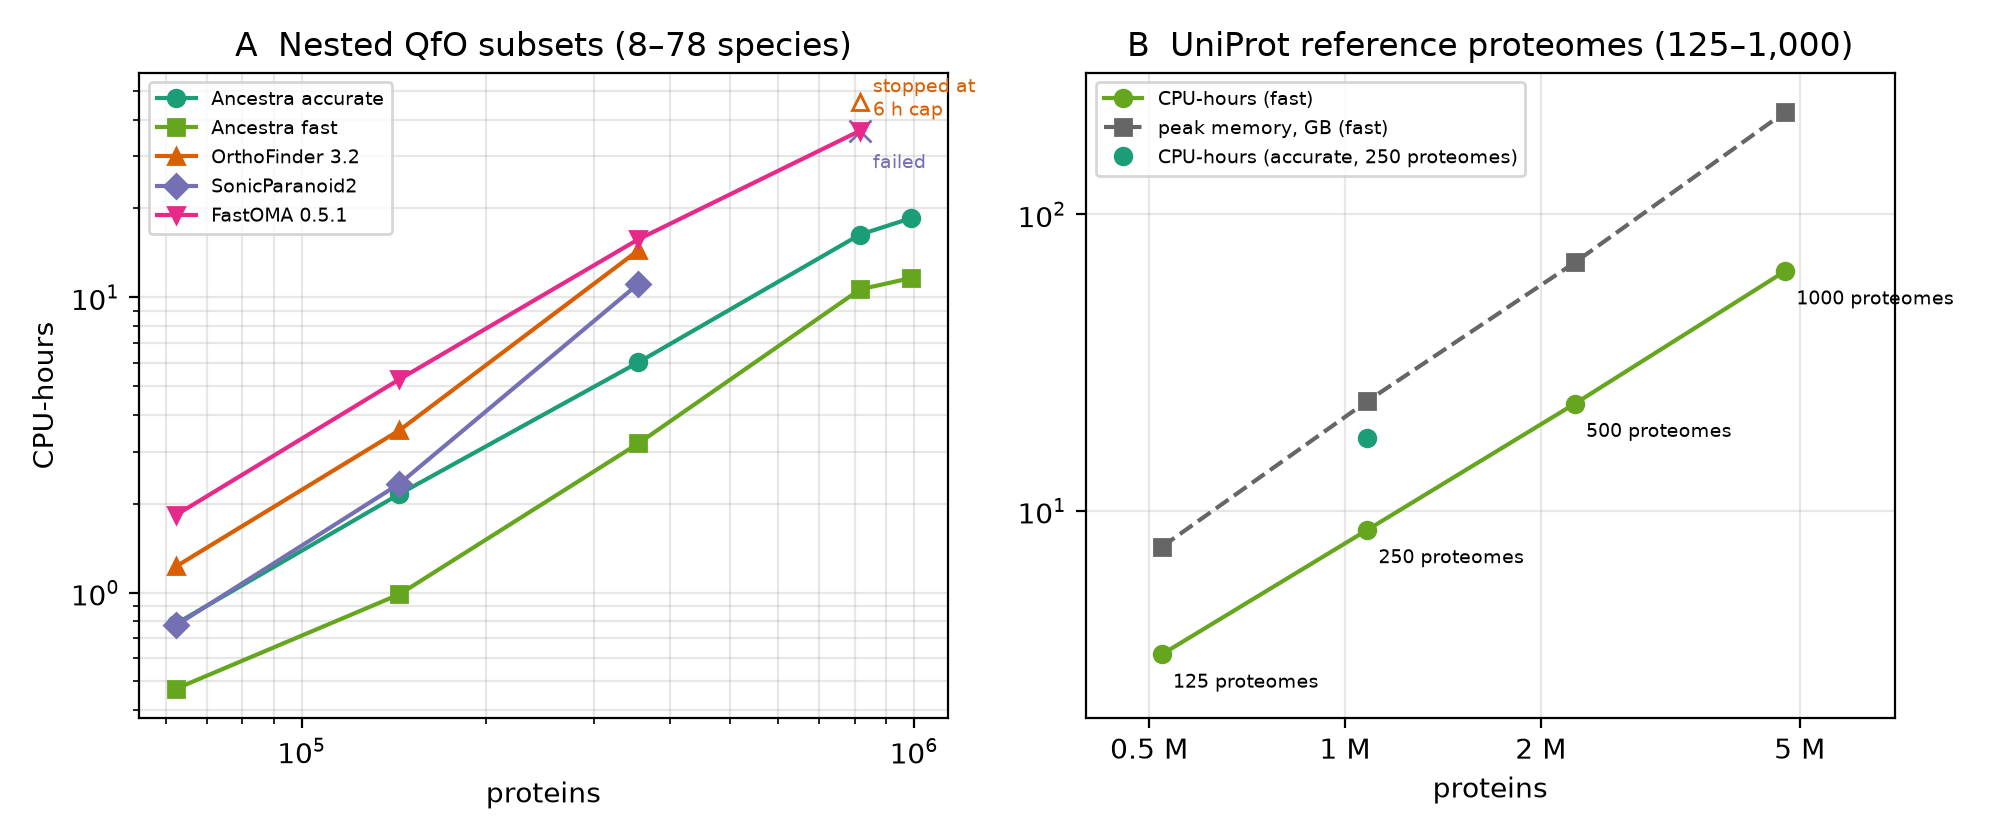
\includegraphics[width=\linewidth]{../docs/figures/fig3_scaling.png}
\caption{{\bf CPU time against number of proteins.} (A) Nested QfO subsets, 8 threads. OrthoFinder at 64 species was stopped at the 6-hour cap (open triangle, lower bound); SonicParanoid2 at 64 species failed (cross). (B) Ancestra on 125--1,000 UniProt reference proteomes, 12 threads; peak memory in GB is shown on the same axis. Measured points only; single runs on a shared node.}
\label{fig:scaling}
\end{figure}

\subsection*{GPU acceleration}
After the method was frozen, the project moved to a node with an NVIDIA A100 GPU. We tested GPU options for each stage, as opt-in code on a separate branch, and evaluated them on development data only. Scoring inside families (S2) takes 60--75\% of the wall time, so it was the main target.
\begin{itemize}
\item \textbf{MMseqs2-GPU}~\cite{kallenborn2025mmseqs2gpu} was slower than DIAMOND on CPU for our searches. Its GPU prefilter needs about 9 ms per query, so it suits a few queries against a large database rather than all-against-all searches of $10^4$--$10^6$ proteins. DIAMOND 2.2.8 has no GPU support.
\item \textbf{GPU Smith--Waterman.} We wrote a CUDA Smith--Waterman kernel (600--640 billion cell updates per second), which reproduces a CPU reference exactly and runs deterministically. With families of up to 1,000 genes on the GPU and larger families on DIAMOND at the same time, S2 was 1.2--1.3 times faster and the whole run 1.18 times faster (OrthoBench \texttt{accurate}: 1,027 vs 1,207 s). Accuracy was unchanged within noise (development OG-F 80.2 vs 79.7, $\Delta$ $+0.5$ \CI{$-3.5$}{$+3.3$}; QfO TreeFam-A development TPR/PPV 0.614/0.929 vs 0.615/0.922).
\item \textbf{All families on the GPU} cut QfO CPU time 16-fold (0.55 vs 9.05 CPU-hours for scoring and merge) but was not equivalent: OrthoBench development OG-F fell by 5.3 \CI{$-12.0$}{$-0.7$} and QfO PPV by 0.016. 78--85\% of DIAMOND's time goes to a few families with more than 1,000 genes, and exhaustive alignment of these families changes the score graph. Not only the number of edges matters. Against the CPU path without cross-family rescue, GPU scores on exactly DIAMOND's pair set also cost 9.1 OG-F. A control shows how sensitive this benchmark is: multiplying the CPU scores by 1\% random noise cost 3.2--7.3 development OG-F over three seeds, although two of the three intervals include 0 and TreeFam-A barely moved. Sparsifying the GPU graph (keep a pair if its score is at least 0.207 times the query's best hit in that species) gave QfO TreeFam-A development TPR/PPV of 0.637/0.930, against 0.615/0.922 on the CPU path (the CIs of both differences include 0; this was the best of seven arms). It needed an estimated 15 times fewer CPU-hours (plus 0.2--0.3 GPU-hours). But it lost 8.4 OrthoBench OG-F, so it remains an untested speed option.
\item \textbf{Local gene trees} are not a GPU problem. About 93\% of a FastTree call (in a sample of 20 small jobs) is the maximum-likelihood optimisation of a small tree, not process start-up. Batching the calls (\texttt{FastTree -n}) saved only 1.6\% of merge time.
\item \textbf{ProstT5 on GPU}~\cite{heinzinger2024prostt5} predicted 3Di at 6,100--7,300 residues per second, 40--60 times faster than on CPU, with 99.9\% agreement with CPU predictions. It filled the 3Di gap for all 48,903 OrthoBench proteins without AlphaFold DB structures in under two hours. This makes complete structure coverage practical, although structure did not improve the final groups.
\item \textbf{ESM-2 embeddings with FAISS nearest-neighbour search}~\cite{lin2023esm2,douze2026faiss} took about 10 minutes for OrthoBench. They could place up to 85\% of development RefOGs in one family (k = 25), above the sequence ceiling of 82\%, but 42\% of neighbours fell outside the protein's family. This is a lead for future work, not a validated component.
\end{itemize}
In short, the GPU gave a modest, accuracy-neutral speed-up. A larger speed-up would need a merge that is robust to the density of the score graph, which is a change of method that we did not make.

\section*{Discussion}
Ancestra shows that HOGs can be built by reconstructing ancestral genes level by level, within families, without a reference database, and that the approach runs on 1,000 proteomes on one node. The cost is not linear: its exponent rose from 1.16 on QfO to 1.35 between 0.5 and 4.75 million proteins, the family step grew fastest, and memory (221 GB at 1,000 proteomes) is the first limit to larger inputs. On OrthoBench it had the highest F of the methods we tested (not significantly above OrthoFinder or SonicParanoid2). It was significantly better than OMA-based resources and ProteinOrtho, and cheaper than OrthoFinder. On QfO its recall was non-inferior to FastOMA and OMA pairs, but below that of OrthoFinder, SonicParanoid2 and InParanoid.

\textbf{Main weakness: deep nodes.} At the deepest levels of the species tree, the merge relies on score rules, often without an outgroup. Rules strict enough to keep OrthoBench orthogroups apart split true orthologs across Eukaryota; looser rules fuse groups. OrthoFinder avoids this by inferring a tree for the whole orthogroup and rooting it with duplication information~\cite{emms2017stride,emms2019orthofinder}. Possible fixes for Ancestra are outgroup tests with a third clade, larger local trees at deep nodes, and a family partition that is not limited by pairwise sequence hits.

\textbf{Extra data layers.} Our clearest finding is negative: a layer can be informative on its own yet add nothing to good sequence-based inference. Gene order and structure each passed their standalone tests with shuffled controls. Neither improved the final groups on held-out data, and structure lowered their precision. A second round of layers (interaction networks, protein abundance, domain architecture, protein language models, intron positions) also failed on development data. Interaction data were too sparse. The other layers mostly separate orthologs from distant homologs, and that evidence is also shared by close paralogs. The cases where these layers add unique information are the cases where they are weakest: gene order decays at deep nodes, and structure is shared by paralogs. Genome sequence was most useful for validation: it exposed our own fission errors.

\textbf{Benchmarks.} The two benchmarks gave different rankings, and the OrthoBench test set was too small for firm conclusions (95\% intervals of about $\pm$12 F points). We report every pre-registered verdict as written, including the failures. Several deviations weaken the evidence: the development data were reused heavily, the TreeFam-A development split was created after the first QfO evaluation, and OMA-based comparators had seen the benchmark species (S3 Text).

\textbf{Running the project with AI agents.} The agent setup made it practical to test many ideas within 48 hours: about 30 approaches were tried and dropped (S1 Text). Three practices helped the most:
\begin{itemize}
\item pre-registering decision rules before seeing results;
\item using shuffled controls for every data layer;
\item having results recomputed by an agent that did not produce them.
\end{itemize}
Independent verification found real errors: a false statement in our list of disclosures, an omitted primary endpoint and confidence intervals that were too narrow. A later check of this manuscript found that three pre-registered QfO comparators were missing from the main text; we added them. The main weakness of the setup was the pressure to tune on a small development set; several gains on development data did not replicate.

\textbf{Limitations.} Run times come from single runs on shared nodes, and no competitor was run beyond 64 species; OrthoFinder hit our time cap and SonicParanoid2 failed at that size. Our simulator was written in-house and not validated against an independent simulator. The merge is slightly sensitive to the order of children in the guide tree (18 OrthoBench orthogroups differ). Development OG-F on OrthoBench is also sensitive to small changes in the scores. A 1\% random jitter lowered it by 3--7 points (three seeds, two intervals include 0), while TreeFam-A barely changed. The parameters were tuned on this benchmark. Of the 81 claims in our claim ledger, which covers results up to the freeze, 22 were independently recomputed; the others were checked against their evidence files. Post-freeze GPU and second-round results were checked separately.

\section*{Materials and methods}

\subsection*{Agent setup}
The project ran in Claude Code with Claude Opus 5.5 as principal investigator (PI). The PI did not write method code itself. It split the project into sub-tasks, each with its own benchmark, and delegated them to subagents: Claude Opus 5.5 for literature, data acquisition, design, algorithm and verification work, and Claude Sonnet 5.5 for the software environment, competitor and scaling runs, bookkeeping and reference checks. Subagents ran in the background, often several at once, and reported back to the PI, which reviewed results, decided next steps and committed them to git.

The research record was kept in plain files:
\begin{itemize}
\item a research tree with every experiment and decision;
\item a list of process lessons;
\item a pre-registered design document, revised in two review rounds by eight reviewer subagents;
\item a ledger of quantitative claims with their evidence files;
\item a list of protocol deviations.
\end{itemize}
Key results were recomputed by a subagent that had not produced them. The PI checked the clock against a 48-hour budget at each milestone.

After the initial prompt, humans gave seven further instructions (S2 Text, section 2). They suggested the Foldcomp structure databases, required at least one OMA resource in every comparison, and paused the project to move it to a node with a GPU. They then asked the agent to test the GPU and resume, kept the 48-hour deadline but made it soft and asked for a fixed header in the repository READMEs, requested this manuscript, and asked for a second round of data layers. Compute was a shared 24-core node for the first 19.5 hours, then a node with 48 cores, 500 GB of memory and one NVIDIA A100 GPU.

\subsection*{Pre-registered protocol}
Before any results, the design document fixed:
\begin{itemize}
\item \textbf{Splits.} OrthoBench RefOGs were split by homology component into development (34) and test (36) halves, so that paralogous RefOGs fall on the same side. This split replaced a first, random split that a reviewer found leaky; three early S0 configurations had been scored by then (S1 Text, section 9.1). For QfO, at most three evaluations were allowed before the method was frozen.
\item \textbf{Success rule.} Ancestra is \emph{comparable} to a method if the lower 95\% bound of the difference is at least $-0.03$ (non-inferiority~\cite{piaggio2012consortnoninferiority}). Without a confidence interval, the verdict is inconclusive.
\item \textbf{Statistics.} Paired bootstrap~\cite{efron1979bootstrap} over RefOGs or reference families, 2,000 resamples, seed 11.
\item \textbf{Layer tests.} Every data layer has a shuffled control and a keep rule written before the test.
\end{itemize}
A TreeFam-A development split (30\% of families) was added after the first QfO evaluation. This and 18 other deviations are listed in S3 Text.

\subsection*{Implementation and freeze}
Ancestra is written in Python and calls DIAMOND 2.2.8, MMseqs2 18, FAMSA and FastTree. The family partition is deterministic: we fixed input order, DIAMOND block sizes, edge order and the Leiden seed, after an early version gave different partitions at different thread counts. The method was frozen (git tag \texttt{freeze-v1}, with hashes of all modules) before the final evaluations. Presets: \texttt{accurate} (default) uses FastTree local trees; \texttt{fast} uses neighbour joining and species-overlap structure.

\subsection*{Benchmarks and comparators}
\begin{itemize}
\item \textbf{OrthoBench:} official Open OrthoBench scoring~\cite{emms2020orthobench}. We ran OrthoFinder 3.2, SonicParanoid2, ProteinOrtho and FastOMA 0.5.1 locally. OMA browser HOGs (release All.May2026) were mapped to OrthoBench identifiers and cut at Bilateria.
\item \textbf{QfO 2022:} the official benchmark code, run locally on the 78-species reference set~\cite{altenhoff2024qfo}; competitor values are published submissions.
\item \textbf{Scaling:} nested, domain-stratified subsets of QfO, one run per point, CPU time from \texttt{/usr/bin/time}; competitors capped at 6 hours of wall time. The large-scale sets are 1,000 UniProt 2026\_03 reference proteomes (800 bacterial, 100 archaeal and 100 eukaryotic; one per genus, phyla visited in a seeded random round-robin), taken in nested subsets of 125, 250, 500 and 1,000, with guide trees from the NCBI taxonomy. Outputs were checked with our OrthoXML validator.
\end{itemize}

\subsection*{Data layers}
\begin{itemize}
\item \textbf{Gene order:} Ensembl 99 annotations~\cite{yates2019ensembl} (OrthoBench) and QfO gene coordinates.
\item \textbf{Structure:} AlphaFold DB 3Di sequences via Foldseek and Foldcomp databases~\cite{vankempen2024foldseek,kim2023foldcomp,varadi2024alphafolddb}.
\item \textbf{Expression:} Bgee~\cite{bastian2025bgee}.
\item \textbf{Isoforms:} Ensembl 99 peptide sets.
\item \textbf{Genome DNA:} miniprot~\cite{li2023miniprot} searches of Ensembl 99 genomes at loci predicted by gene order.
\item \textbf{Second round (post-freeze, development data only):}
  \begin{itemize}
  \item STRING v12, using only each organism's own experimental and co-expression channels, since transferred evidence is itself derived from orthology;
  \item hu.MAP 3.0 and PaxDb 5.0;
  \item Pfam-A 38.2 (\texttt{hmmsearch --cut\_ga});
  \item ESM-2 and ProtT5 embeddings, and a contrastive head trained on synteny-supported pairs from families with no development or test genes;
  \item intron positions from Ensembl 99 GFF3;
  \item ProstT5 3Di predicted on a GPU.
  \end{itemize}
  Five agents ran these in parallel under one shared protocol: pre-registered arms and keep rules, and shuffled controls with seeds 11, 23 and 47.
\end{itemize}
Details of each sub-task benchmark are in the research repository (\texttt{docs/S*\_*.md}, \texttt{docs/L2\_*.md}).

\section*{Data and code availability}
Code, predictions (OrthoXML, pairs and orthogroups for OrthoBench and QfO), a runnable example and the original task prompt are in the accompanying repository (URL to be added by the human authors on publication). The full research record, including all failed experiments, is in the research repository.

\section*{Supporting information}

\paragraph*{S1 Text.}
\label{S1_Text}
{\bf Methods and design choices that did not work.}

\paragraph*{S2 Text.}
\label{S2_Text}
{\bf Original task prompt given to the agent.}

\paragraph*{S3 Text.}
\label{S3_Text}
{\bf Protocol deviations and independent verification.}

\paragraph*{S1 Table.}
\label{S1_Table}
{\bf Full QfO 2022 results for all 20 published methods and both Ancestra presets.}

\section*{Acknowledgments}
The project was run as part of a hackathon of the Beltrao lab at ETH Zurich.

\nolinenumbers

\bibliography{references}

\end{document}
